\subsection{\ours Overview}
\label{sec:overview}

\begin{figure*}[t]
    \centering
    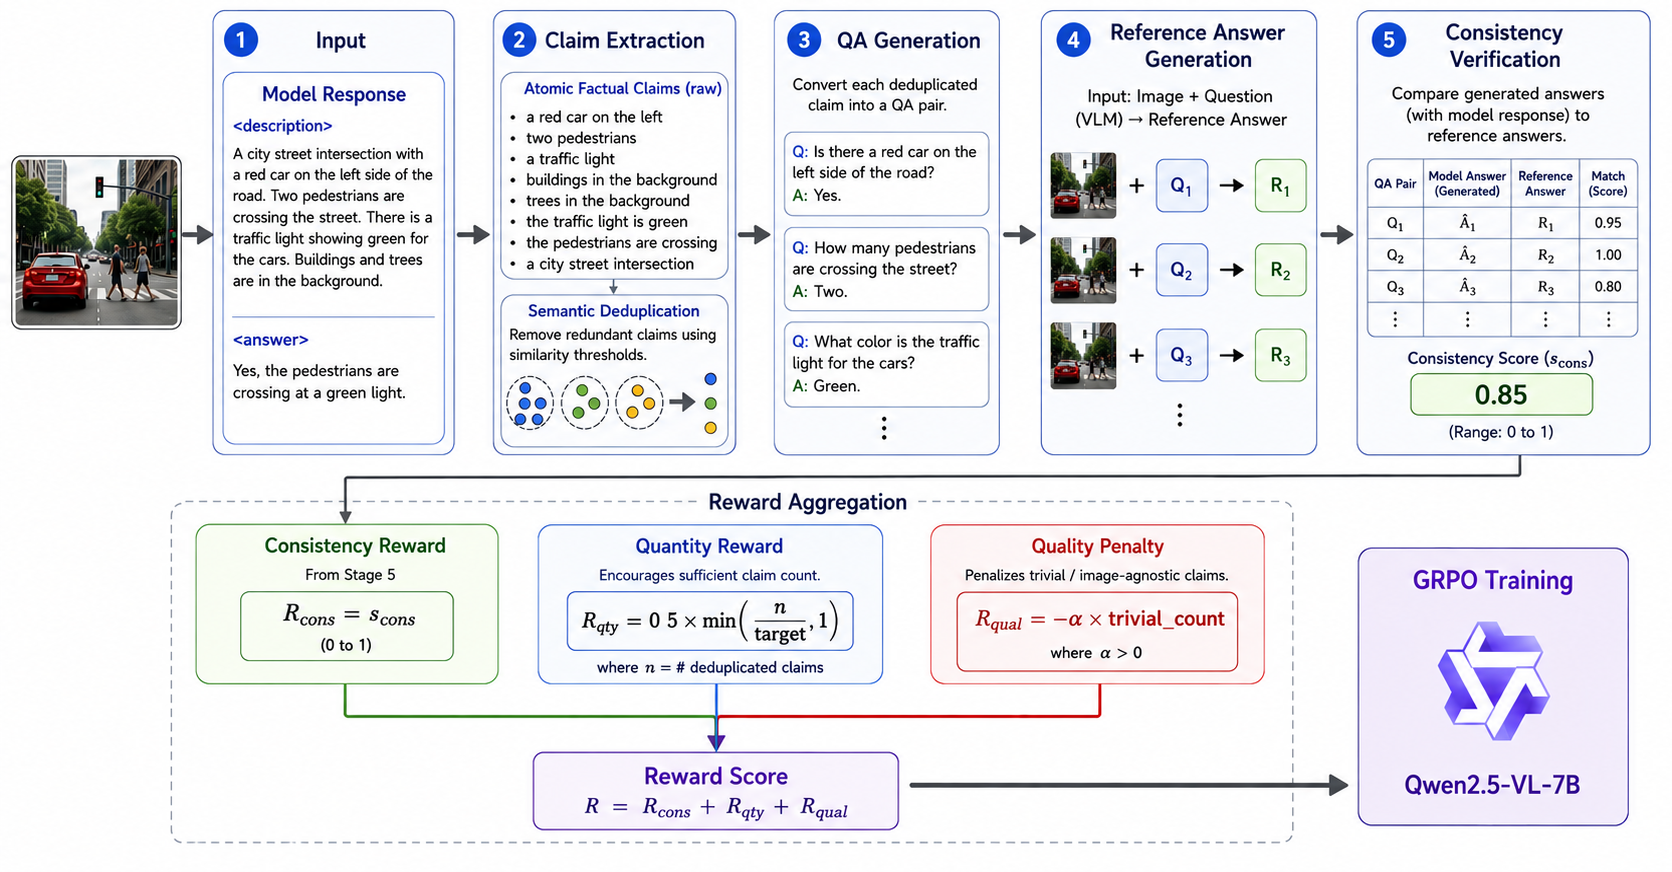
\includegraphics[width=\textwidth]{figures/pipeline.png}
    \caption{Overview of the \ours pipeline. Given a model-generated response,
    \ours first extracts atomic factual claims from the generated description
    and removes semantically redundant claims. Each remaining claim is converted
    into a visual question-answer pair, where the answer is implied by the
    generated description. The VLM then answers the same questions using the
    original image, producing image-grounded reference answers. The consistency
    between the implied answers and the reference answers is verified through
    majority voting. In addition, Visual Evidence Calibration (VEC) calibrates
    the reward by encouraging diverse claims, rewarding sufficient claim
    coverage, and penalizing claims answerable from degraded visual evidence.}
    \label{fig:pipeline}
\end{figure*}

The core idea of \ours is to convert open-ended visual factuality evaluation
into a set of fine-grained answer consistency checks. Rather than directly
asking a model to judge whether an entire generated response is correct, \ours
first decomposes the description into atomic claims, transforms each claim into
a visual question-answer pair, obtains an image-grounded reference answer, and
then verifies whether the claim-implied answer is consistent with the
image-grounded answer.

This design introduces an information asymmetry between generation and
verification. The model-generated description provides the claim-implied answer,
while the reference answer is obtained by querying the VLM with the image and the
corresponding visual question. The final verifier compares two answers rather
than re-reading the full generated description, reducing the risk that the model
simply confirms its own hallucinated text.

Formally, \ours constructs a self-verifying reward
\begin{equation}
    R_{\mathrm{SV}}(I,q,y)
\end{equation}
from the generated description $y^{\mathrm{desc}}$. This reward consists of a
claim-level consistency score and a Visual Evidence Calibration term:
\begin{equation}
    R_{\mathrm{SV}}(I,q,y)
    =
    R_{\mathrm{cons}}
    +
    R_{\mathrm{VEC}}.
\end{equation}
The following sections describe the construction of $R_{\mathrm{cons}}$ and
$R_{\mathrm{VEC}}$.

\subsection{Claim-Level Self-Verification}
\label{sec:claim_level_verification}

\paragraph{Claim Extraction.}
Given the generated description $y^{\mathrm{desc}}$, \ours first extracts a set
of atomic factual claims:
\begin{equation}
    \mathcal{C}
    =
    \{c_1,c_2,\ldots,c_m\}
    =
    \mathrm{Extract}(y^{\mathrm{desc}}).
\end{equation}
Each claim $c_i$ is a short, self-contained statement about a single visual
fact, such as object existence, color, quantity, attribute, action, or spatial
relation. For example, from the sentence
\textit{``A red car is parked on the left side of the road''}, the extracted
claims may include \textit{``there is a car''}, \textit{``the car is red''}, and
\textit{``the car is on the left side of the road''}. This decomposition enables
fine-grained verification instead of coarse response-level judgment.

\paragraph{Semantic Deduplication.}
The raw claim set may contain repeated or semantically overlapping claims.
Directly using all claims for reward computation can encourage reward hacking,
where the model repeats the same correct fact to increase the reward. Therefore,
we apply semantic deduplication before question generation.

Each claim is encoded by a sentence encoder $\phi(\cdot)$, and the semantic
similarity between two claims is computed as
\begin{equation}
    \mathrm{sim}(c_i,c_j)
    =
    \frac{
    \phi(c_i)^\top \phi(c_j)
    }{
    \|\phi(c_i)\|\cdot\|\phi(c_j)\|
    }.
\end{equation}
If $\mathrm{sim}(c_i,c_j)$ exceeds a threshold, the two claims are treated as
duplicates and only one representative is retained. In practice, we use
type-aware thresholds: claims of the same type are deduplicated more
aggressively, while claims of different types are retained unless their
similarity is sufficiently high. The resulting deduplicated claim set is denoted
as
\begin{equation}
    \mathcal{C}^{\ast}
    =
    \{c_1^{\ast},c_2^{\ast},\ldots,c_n^{\ast}\},
    \quad n\leq m.
\end{equation}

\paragraph{Question-Answer Generation.}
For each deduplicated claim $c_i^{\ast}$, \ours generates a visual
question-answer pair:
\begin{equation}
    (v_i,a_i)
    =
    \mathrm{QA}(c_i^{\ast}),
\end{equation}
where $v_i$ is a visual question and $a_i$ is the answer implied by the claim.
For instance, the claim \textit{``the traffic light is green''} can be
transformed into the question \textit{``What color is the traffic light?''} with
the implied answer \textit{``green''}. We denote the set of generated QA pairs as
\begin{equation}
    \mathcal{Q}
    =
    \{(v_i,a_i)\}_{i=1}^{n}.
\end{equation}

\paragraph{Reference Answer Generation.}
Next, \ours obtains image-grounded reference answers by querying the VLM with
the original image $I$ and the generated questions:
\begin{equation}
    a_i^{\prime}
    =
    \mathrm{Ans}(I,v_i),
    \quad i=1,\ldots,n.
\end{equation}
Here, $a_i$ is the answer implied by the generated description, whereas
$a_i^{\prime}$ is the reference answer grounded in the input image. This
separation is central to the asymmetric verification design: the reference
answer is generated from the image-question pair rather than from the original
description.

\paragraph{Answer Consistency Verification.}
Finally, \ours verifies whether the claim-implied answer $a_i$ is consistent
with the image-grounded reference answer $a_i^{\prime}$. We use a verifier
$f_{\mathrm{ver}}$ to compare the two answers:
\begin{equation}
    z_i
    =
    f_{\mathrm{ver}}(a_i,a_i^{\prime})
    \in
    \{0,1\},
\end{equation}
where $z_i=1$ indicates that the two answers are semantically consistent. For
robustness, the verification is performed multiple times and aggregated by
strict majority voting:
\begin{equation}
    z_i
    =
    \mathbbm{1}
    \left[
    \sum_{k=1}^{K} z_i^{(k)} > \frac{K}{2}
    \right],
\end{equation}
where $K$ is the number of verification votes. The claim-level consistency
reward is then computed as
\begin{equation}
    R_{\mathrm{cons}}
    =
    \frac{1}{n}
    \sum_{i=1}^{n}
    z_i.
\end{equation}
This reward measures the fraction of deduplicated claims that are supported by
the image-grounded reference answers.

\subsection{Visual Evidence Calibration}
\label{sec:vec}

Although claim-level verification provides fine-grained reward signals, the
self-generated reward can still be exploited by degenerate behaviors. The model
may repeat similar claims, produce too few informative claims, or generate
trivial claims that can be answered without looking at the image. To improve the
reliability of the reward, we introduce \textit{Visual Evidence Calibration}
(VEC), which calibrates the self-verifying reward through three mechanisms:
redundancy control, informativeness reward, and visual-dependence penalty.

\paragraph{Redundancy Control.}
The first component of VEC is the semantic deduplication described above.
Although deduplication occurs before QA generation, its role is reward
calibration: it prevents repeated claims from being counted multiple times in
the final consistency reward. Therefore, the consistency score is computed only
over the deduplicated claim set $\mathcal{C}^{\ast}$ rather than the raw claim
set $\mathcal{C}$.

\paragraph{Informativeness Reward.}
A model can also obtain a stable consistency score by producing very few claims.
Such responses may be accurate but under-informative. To encourage sufficient
visual coverage, we add a claim count reward:
\begin{equation}
    R_{\mathrm{cnt}}
    =
    \lambda_{\mathrm{cnt}}
    \cdot
    \min
    \left(
    \frac{n}{n_{\mathrm{target}}},
    1
    \right),
\end{equation}
where $n$ is the number of deduplicated claims,
$n_{\mathrm{target}}$ is the target number of claims, and
$\lambda_{\mathrm{cnt}}$ controls the maximum value of the reward. In our
implementation, $\lambda_{\mathrm{cnt}}=0.5$, so this term encourages
informativeness while keeping factual consistency as the dominant signal.

\paragraph{Visual-Dependence Penalty.}
Some claims may be easy to answer even without meaningful visual evidence. For
example, generic claims such as \textit{``there are objects in the image''} may
often be answered correctly from language priors alone. To identify such
image-agnostic claims, we introduce a degraded-image test.

We construct a degraded version $\tilde{I}$ of the original image by applying
heavy Gaussian blur, grayscale conversion, and horizontal flipping. The same
question $v_i$ is then answered using $\tilde{I}$:
\begin{equation}
    \tilde{a}_i
    =
    \mathrm{Ans}(\tilde{I},v_i).
\end{equation}
If the degraded-image answer $\tilde{a}_i$ is consistent with the original-image
reference answer $a_i^{\prime}$, and neither answer is unknown, the claim is
marked as trivial:
\begin{equation}
    t_i
    =
    \mathbbm{1}
    \left[
    f_{\mathrm{ver}}(\tilde{a}_i,a_i^{\prime})=1
    \land
    a_i^{\prime}\neq \mathrm{unknown}
    \land
    \tilde{a}_i\neq \mathrm{unknown}
    \right].
\end{equation}
The quality penalty is defined as
\begin{equation}
    R_{\mathrm{qual}}
    =
    -
    \lambda_{\mathrm{qual}}
    \sum_{i=1}^{n} t_i,
\end{equation}
where $\lambda_{\mathrm{qual}}>0$ is the penalty coefficient. This penalty
discourages claims whose answers remain unchanged even when visual evidence is
severely degraded, pushing the model toward claims that require genuine image
grounding.

\paragraph{VEC Reward.}
The overall VEC term is
\begin{equation}
    R_{\mathrm{VEC}}
    =
    R_{\mathrm{cnt}}
    +
    R_{\mathrm{qual}},
\end{equation}
with redundancy control implicitly applied through the deduplicated claim set
$\mathcal{C}^{\ast}$.

\subsection{Final Reward and Training}
\label{sec:final_reward}

The final reward used for GRPO training is
\begin{equation}
    R_{\mathrm{SV}}(I,q,y)
    =
    R_{\mathrm{cons}}
    +
    R_{\mathrm{cnt}}
    +
    R_{\mathrm{qual}}.
\end{equation}
Equivalently, we use
\begin{equation}
    r(I,q,y)=R_{\mathrm{SV}}(I,q,y)
\end{equation}
as the reward signal in GRPO.

The three reward components are complementary. $R_{\mathrm{cons}}$ encourages
the generated description to be factually consistent with the image;
$R_{\mathrm{cnt}}$ encourages the model to provide sufficiently informative and
coverage-rich descriptions; and $R_{\mathrm{qual}}$ penalizes claims that can be
answered from degraded visual evidence rather than genuine image understanding.
Together, they provide a scalable annotation-free reward for hallucination
mitigation.

During training, for each image-instruction pair $(I,q)$, the policy first
generates a group of responses. For each response, \ours extracts and
deduplicates claims, generates QA pairs, obtains image-grounded reference
answers, verifies answer consistency through majority voting, and applies VEC to
calibrate the reward. The resulting rewards are normalized within the group and
used to update the policy with GRPO.
